\chapter{Caso d'uso}\label{chp:05-usecase}
In questo capitolo è descritto un esempio di come l'utente può interagire con la piattaforma di Moon Cloud e di come reagisce 
il sistema di raccomandazione alle sue azioni.
%
\section*{Primi passi su Moon Cloud}
\begin{figure}[ht!]
    \centering
    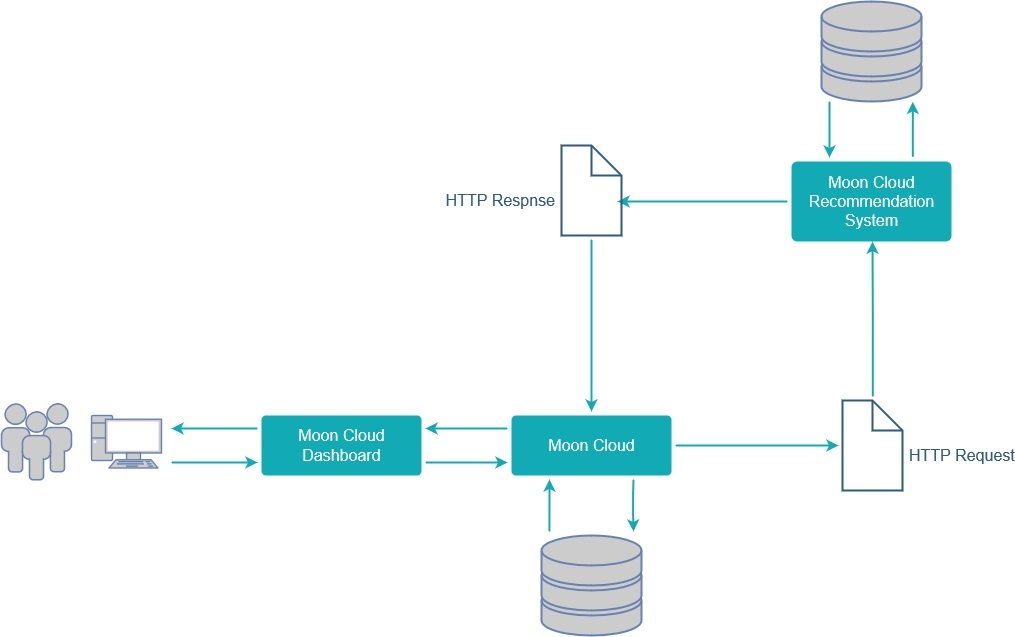
\includegraphics[scale=0.52]{images/UML_MoonCloud_HowToDo.jpg}
    \caption[Schema di funzionamento di questa soluzione]{Schema di funzionamento congiunto tra Moon Cloud e il sistema di raccomandazione.}
    \label{fig:UML_MoonCloud_HowToDo}
\end{figure}
\hfill\break
Una volta implementato quanto proposto in questa tesi e integrato col sistema di Moon Cloud, nel momento in cui un utente 
accede ai servizi offerti da questo framework, completa la propria registrazione, una copia dei suoi dati dal database di 
Moon Cloud verrà anche fatta nel database usato per poter effettuare il processo di recommendation. Questa operazione di 
copia dei dati da un database a un altro viene fatta per poter avere i dati consistenti in entrambi i punti così da 
fornire al'utente delle raccomandazioni affidabili. Tutto questo viene fatto non solo per i dati degli utenti ma anche 
per i Controlli e le Evaluation. Dalla Figura \ref{fig:UML_MoonCloud_HowToDo} è possibile osservare come interagiscon 
ad alto livello la piattaforma Moon Cloud e il modulo del sistema di raccomandazione.\hfill\break
Inizialmente un nuovo utente, che ha appena effettuato la registrazione e avuto accesso alla propria dashboard, (l'interfaccia 
web) per poter schedulare e lanciare delle Evaluation, egli deve inserire uno o più Target (asset che l'utente possiede e su 
cui vuole essere certo che vengano rispettate certe politiche di sicurezza o garantiti certi standard).
%
\section*{Target Recommendation}
Nel momento in cui viene inserito il primo Target, del quale sarà specificato un Target Type (\textit{Url}, \textit{Host Windows}, 
\textit{Host Linux}, \textit{Azure} o \textit{AWS}), verra richiamato tramite l'apposita API REST (HTTP Request, method: GET, URL: \\
\texttt{recommendation/target/<target\_type\_id>/}) il \textit{Target Recommendation Algorithm}, il quale restituirà una 
risposta HTTP contenente, in formato JSON, una lista delle Evaluation ritenute più adatte per il Target specificato. 
La lista ottenuta dalla chiamata all'algoritmo restiuisce soltanto un valore corrispondente a un 
identificatore univoco (\texttt{other\_id}) delle Evaluation sia nel database effettivo di Moon Cloud sia nel database usato 
per i processi di recommendation. Nel caso in cui l'utente ha inserito un Target di tipo \textit{Host Linux}, l'URL della 
richiesta sarà \texttt{/recommendation/target/1/}, e nel Listing \ref{lst:rsp_Target_alg} è possibile trovare il body 
della risposta HTTP.
\lstset{style=python_code_style}
\begin{lstlisting}[language=Python, label=lst:rsp_Target_alg, caption={Esempio del body della risposta HTTP alla chiamata del 
    \textit{Target Recommendation Algorithm}}]
[
    {"other_id": 25},
    {"other_id": 29},
    {"other_id": 30},
    {"other_id": 24},
    {"other_id": 28},
    {"other_id": 31},
    {"other_id": 23},
    {"other_id": 26}
]
\end{lstlisting}
%
\section*{Item Recommendation}
Una volta che un utente ha fornito a Moon Cloud i Target che vuole proteggere, può iniziare a configurare per quel Target uno 
o più processi di Evaluation, per ognuna delle quali scelte è possibile effettuare una richiesta all'apposita API REST, 
attraverso l'URL \texttt{recommendation/item/<item\_other\_id>/} al \textit{Item Recommendation Algorithm}, il quale 
restituirà una risposta HTTP contenente, in formato JSON, una lista delle Evaluation ritenute più simili a quella selezionata 
dall'utente. Nel caso in cui sia stata scelta l'Evaluation \textit{Macie Scanner}, con relativo \texttt{other\_id} pari a 34, 
verrà restituita la lista mostrata nel Listing \ref{lst:rsp_item_alg}; il quale 
contiene le Evaluation, con \texttt{other\_id} pari a 35 e 36, i quali corrispondono rispettivamente a \textit{Sqs Checker} 
e \textit{Inspector Vulnerability Scan}, entrambe sono applicabili a sistemi AWS.
\begin{lstlisting}[language=Python, label=lst:rsp_item_alg, caption={Esempio del body della risposta HTTP alla chiamata del 
    \textit{Item Recommendation Algorithm}}]
[
    {"other_id": 35},
    {"other_id": 36}
]
\end{lstlisting}
%
\section*{User and Hybrid Recommendation}
Nel momento in cui più utenti iniziano a utilizzare Moon Cloud e a proteggere i propri asset, schedulando e configurando 
processi di Evaluation, sarà possibile per un utente fornirgli delle raccomandazioni sulla base anche delle Evaluation usate da 
altri utenti. Per poter determinare ciò è necessario richiamare tramite l'apposita API REST, con URL: \\
\texttt{recommendation/user/<user\_other\_id>/} lo \textit{User Recommendation Algorithm}, il quale restituirà una 
risposta HTTP contenente, in formato JSON, una lista delle Evaluation ritenute più adatte per l'utente indicato. 
Nel caso di un utente, con \texttt{other\_id} pari a 10, e che ha utilizzato le seguenti Evaluation: \textit{Availability Check},
\textit{Pen Tester} e \textit{Macie Scanner}, l'URL della richiesta sarà 
\texttt{/recommendation/user/10/}, e nel Listing \ref{lst:rsp_user_alg} è possibile trovare il body della risposta HTTP; il quale 
contiene l'Evaluation, con \texttt{other\_id} pari a 36, la quale corrisponde a \textit{Inspector Vulnerability Scan} il quale 
è compatibile con \textit{Macie Scanner} perché entrambi sono applicabili a sistemi AWSS.
\begin{lstlisting}[language=Python, label=lst:rsp_user_alg, caption={Esempio di risposta HTTP alla chiamata del 
    \textit{User Recommendation Algorithm}}]
[
    {"other_id": 36}
]
\end{lstlisting}
Inoltre è possibile richiamare sempre per un utente, tramite lo stesso procedimento descritto per i casi precedenti, 
l' \textit{Hybrid Recommendation Algorithm}, il quale oltre a determinare delle Evaluation compatibili, usate da altri 
utenti, con quelle usate dal utente preso in considerazione, andrà a recuperare tutte quelle che non sono state ottenute con lo
\textit{User Recommendation Algorithm} attraverso un'applicazione dell'\textit{Item Recommendation Algorithm}. Nel caso di 
un utente, con \texttt{other\_id} pari a 10, l'URL della richiesta sarà 
\texttt{/recommendation/hybrid/10/}, e nel Listing \ref{lst:rsp_hybrid_alg} è possibile trovare il body della risposta HTTP.
\begin{lstlisting}[language=Python, label=lst:rsp_hybrid_alg, caption={Esempio di risposta HTTP alla chiamata del 
    \textit{Hybrid Recommendation Algorithm}}]
[
    {"other_id": 23},
    {"other_id": 24},
    {"other_id": 25},
    {"other_id": 26},
    {"other_id": 28},
    {"other_id": 29},
    {"other_id": 30},
    {"other_id": 31},
    {"other_id": 32},
    {"other_id": 35},
    {"other_id": 36},
    {"other_id": 43},
    {"other_id": 45},
    {"other_id": 46},
    {"other_id": 47},
    {"other_id": 48}
]
\end{lstlisting}
